\documentclass[11pt]{article}
\usepackage[utf8]{inputenc}
\usepackage[T1]{fontenc}
\usepackage{lmodern}
\usepackage{amsmath,amssymb,amsthm}
\usepackage{booktabs}
\usepackage{graphicx}
\usepackage{geometry}
\usepackage{caption}
\usepackage{subcaption}
\usepackage{microtype}
\usepackage{hyperref}
\usepackage{natbib}
\usepackage{xurl}
\usepackage{xcolor}

\geometry{margin=1in}
\hypersetup{colorlinks=true, linkcolor=blue!50!black,
            citecolor=green!45!black, urlcolor=blue!55!black}

\title{\bf Polynomial Activations and Projective Normalization:\\[2pt]
An Empirical Study of What Makes Deep\\ Fully-Connected Networks Trainable}

\author{Xiuyi Yang\\ \texttt{fwinlee@gmail.com}}
\date{\today}

\begin{document}
\maketitle

% 代码与全部实验日志：见文末 "Reproducibility and code availability"
\noindent\emph{Code, raw results and paper sources:}
\url{https://github.com/lfwin/Polynomial-Activation-and-projective-normalization}
\vspace{0.6em}

% 所有数字宏（由 experiments/make_macros.py 生成）
% ============================================================
% 由 experiments/make_macros.py 从实验 JSON 自动生成。
% 不要手改：论文中的所有数字都引用这里的宏。
% ============================================================
\newcommand{\LfifteenGeluAcc}{98.13}
\newcommand{\LfifteenIdentityAcc}{92.54}
\newcommand{\LfifteenPolyAcc}{92.96}
\newcommand{\LfifteenPolybnAcc}{96.37}
\newcommand{\LfifteenPolylnAcc}{95.94}
\newcommand{\LfifteenPolyprojAcc}{95.62}
\newcommand{\LfifteenReluAcc}{97.83}
\newcommand{\LfiftyCollapseAcc}{10.28}
\newcommand{\LfiftyIdentityAcc}{89.89}
\newcommand{\LfiftyPolyAcc}{10.28}
\newcommand{\LfiftyPolylnAcc}{11.35}
\newcommand{\LfiftyPolyprojAcc}{11.35}
\newcommand{\LfiftyProjVsReluPt}{0.00}
\newcommand{\LfiftyReluAcc}{11.35}
\newcommand{\LfiftyReluBnAcc}{44.64}
\newcommand{\LfiveGeluAcc}{98.07}
\newcommand{\LfiveIdentityAcc}{92.75}
\newcommand{\LfivePolyAcc}{95.09}
\newcommand{\LfivePolybnAcc}{96.51}
\newcommand{\LfivePolylnAcc}{96.32}
\newcommand{\LfivePolyprojAcc}{95.21}
\newcommand{\LfiveReluAcc}{98.24}
\newcommand{\LtenGeluAcc}{98.20}
\newcommand{\LtenIdentityAcc}{92.71}
\newcommand{\LtenPolyAcc}{94.34}
\newcommand{\LtenPolybnAcc}{96.75}
\newcommand{\LtenPolylnAcc}{96.29}
\newcommand{\LtenPolyprojAcc}{95.93}
\newcommand{\LtenProjVsReluPt}{2.14}
\newcommand{\LtenReluAcc}{98.07}
\newcommand{\LthirtyIdentityAcc}{91.98}
\newcommand{\LthirtyPolyAcc}{10.28}
\newcommand{\LthirtyPolylnAcc}{95.38}
\newcommand{\LthirtyPolyprojAcc}{94.10}
\newcommand{\LthirtyProjVsReluPt}{0.29}
\newcommand{\LthirtyReluAcc}{94.39}
\newcommand{\LthirtyReluBnAcc}{97.39}
\newcommand{\LthreeGeluAcc}{98.19}
\newcommand{\LthreeIdentityAcc}{92.72}
\newcommand{\LthreePolyAcc}{94.04}
\newcommand{\LthreePolybnAcc}{94.85}
\newcommand{\LthreePolylnAcc}{94.91}
\newcommand{\LthreePolyprojAcc}{94.45}
\newcommand{\LthreeReluAcc}{98.03}
\newcommand{\LtwentyGeluAcc}{97.62}
\newcommand{\LtwentyIdentityAcc}{92.45}
\newcommand{\LtwentyPolyAcc}{92.88}
\newcommand{\LtwentyPolybnAcc}{95.83}
\newcommand{\LtwentyPolylnAcc}{96.11}
\newcommand{\LtwentyPolyprojAcc}{95.43}
\newcommand{\LtwentyProjVsReluPt}{2.22}
\newcommand{\LtwentyReluAcc}{97.65}
\newcommand{\LtwoGeluAcc}{97.76}
\newcommand{\LtwoIdentityAcc}{92.68}
\newcommand{\LtwoPolyAcc}{92.81}
\newcommand{\LtwoPolybnAcc}{92.78}
\newcommand{\LtwoPolylnAcc}{93.54}
\newcommand{\LtwoPolyprojAcc}{92.68}
\newcommand{\LtwoReluAcc}{97.61}
\newcommand{\actBandPt}{0.13}
\newcommand{\actNormPolyFirst}{1.00}
\newcommand{\actNormPolyLast}{1.0000}
\newcommand{\actNormPolyRatio}{1}
\newcommand{\actNormReluFirst}{3.45}
\newcommand{\actNormReluLast}{0.1657}
\newcommand{\actNormReluRatio}{0.048}
\newcommand{\actNormSwiFirst}{0.86}
\newcommand{\actNormSwiLast}{0.0000}
\newcommand{\actNormSwiRatio}{0}
\newcommand{\bsplineBestAcc}{98.36}
\newcommand{\bsplineNoneAcc}{98.20}
\newcommand{\chebyBestAcc}{97.89}
\newcommand{\chebyNoneAcc}{11.35}
\newcommand{\dFifty}{50}
\newcommand{\dThirty}{30}
\newcommand{\degFixLamSpanPt}{0.49}
\newcommand{\degGridBestLam}{0.1}
\newcommand{\degGridMaxAcc}{97.46}
\newcommand{\degGridMinAcc}{95.76}
\newcommand{\degLamSpanPt}{1.37}
\newcommand{\degThreeMinAcc}{96.69}
\newcommand{\degTwoMinAcc}{95.93}
\newcommand{\degfiveAcc}{96.69}
\newcommand{\degfiveLamFiveHundredthsAcc}{97.18}
\newcommand{\degfiveLamOneHundredthAcc}{96.69}
\newcommand{\degfiveLamOneTenthAcc}{97.36}
\newcommand{\degfiveLamOneThousandthAcc}{95.76}
\newcommand{\degfourAcc}{96.20}
\newcommand{\degfourLamFiveHundredthsAcc}{97.19}
\newcommand{\degfourLamOneHundredthAcc}{96.20}
\newcommand{\degfourLamOneTenthAcc}{97.46}
\newcommand{\degfourLamOneThousandthAcc}{95.92}
\newcommand{\degthreeAcc}{95.93}
\newcommand{\degthreeLamFiveHundredthsAcc}{96.74}
\newcommand{\degthreeLamOneHundredthAcc}{95.93}
\newcommand{\degthreeLamOneTenthAcc}{97.21}
\newcommand{\degthreeLamOneThousandthAcc}{95.97}
\newcommand{\degtwoAcc}{95.95}
\newcommand{\degtwoLamFiveHundredthsAcc}{96.11}
\newcommand{\degtwoLamOneHundredthAcc}{95.95}
\newcommand{\degtwoLamOneTenthAcc}{97.05}
\newcommand{\degtwoLamOneThousandthAcc}{95.94}
\newcommand{\fidEOneTest}{90.51}
\newcommand{\fidEOneTrain}{87.15}
\newcommand{\fidETwoTest}{92.16}
\newcommand{\fidETwoTrain}{91.52}
\newcommand{\geluNoneAcc}{98.20}
\newcommand{\gluGapPt}{86.6}
\newcommand{\gluLayerMean}{97.98}
\newcommand{\gluNoneMax}{11.35}
\newcommand{\gluNoneMean}{11.35}
\newcommand{\identityNoneAcc}{92.71}
\newcommand{\learnCycles}{10.4}
\newcommand{\legendreBestAcc}{98.03}
\newcommand{\legendreNoneAcc}{11.35}
\newcommand{\lrBase}{0.001}
\newcommand{\nCfgs}{301}
\newcommand{\nGluNone}{3}
\newcommand{\paramElem}{233,866}
\newcommand{\paramGapPct}{2.0}
\newcommand{\paramGate}{238,466}
\newcommand{\polyBatchAcc}{96.75}
\newcommand{\polyDeg}{3}
\newcommand{\polyGap}{1.59}
\newcommand{\polyLam}{0.01}
\newcommand{\polyLayerAcc}{96.29}
\newcommand{\polyLtwoAcc}{95.93}
\newcommand{\polyLtwoDeltaPt}{+1.59}
\newcommand{\polyNoneAcc}{94.34}
\newcommand{\polyNoneToBest}{3.86}
\newcommand{\polyProjAcc}{95.93}
\newcommand{\polyProjToBest}{2.27}
\newcommand{\polyRmsAcc}{96.29}
\newcommand{\refEoneTest}{90.51}
\newcommand{\refEoneTrain}{87.15}
\newcommand{\refEpochSec}{2.0}
\newcommand{\refEpochs}{20}
\newcommand{\refEtwoTest}{91.80}
\newcommand{\refEtwoTrain}{91.09}
\newcommand{\refParams}{233,866}
\newcommand{\refTestAcc}{96.86}
\newcommand{\refTotalSec}{40}
\newcommand{\refTrainAcc}{98.26}
\newcommand{\reluBatchAcc}{98.19}
\newcommand{\reluLayerAcc}{98.11}
\newcommand{\reluLtwoAcc}{97.88}
\newcommand{\reluLtwoDeltaPt}{-0.19}
\newcommand{\reluNoneAcc}{98.07}
\newcommand{\reluRmsAcc}{98.03}
\newcommand{\seedsPolybnMean}{96.83}
\newcommand{\seedsPolybnN}{5}
\newcommand{\seedsPolybnStd}{0.06}
\newcommand{\seedsPolylnMean}{96.15}
\newcommand{\seedsPolylnN}{5}
\newcommand{\seedsPolylnStd}{0.12}
\newcommand{\seedsPolyprojMean}{95.72}
\newcommand{\seedsPolyprojN}{5}
\newcommand{\seedsPolyprojStd}{0.22}
\newcommand{\seedsReluMean}{98.09}
\newcommand{\seedsReluN}{5}
\newcommand{\seedsReluStd}{0.11}
\newcommand{\siluNoneAcc}{98.13}
\newcommand{\synthBlobsBest}{99.38}
\newcommand{\synthBlobsBestName}{identity}
\newcommand{\synthBlobsRelu}{99.38}
\newcommand{\synthCheckerBest}{92.00}
\newcommand{\synthCheckerBestName}{GeGLU}
\newcommand{\synthCheckerRelu}{89.12}
\newcommand{\synthCubesBest}{96.88}
\newcommand{\synthCubesBestName}{relu}
\newcommand{\synthCubesRelu}{96.88}
\newcommand{\synthGausshighdimBest}{35.62}
\newcommand{\synthGausshighdimBestName}{polynomial}
\newcommand{\synthGausshighdimRelu}{6.12}
\newcommand{\synthParityBest}{100.00}
\newcommand{\synthParityBestName}{relu}
\newcommand{\synthParityRelu}{100.00}
\newcommand{\synthRingsBest}{100.00}
\newcommand{\synthRingsBestName}{relu}
\newcommand{\synthRingsRelu}{100.00}
\newcommand{\synthSpiralBest}{77.75}
\newcommand{\synthSpiralBestName}{GeGLU}
\newcommand{\synthSpiralRelu}{72.12}
\newcommand{\synthXorBest}{97.88}
\newcommand{\synthXorBestName}{relu}
\newcommand{\synthXorRelu}{97.88}
\newcommand{\tanhNoneAcc}{97.79}
\newcommand{\wdecay}{0.0001}


\begin{abstract}
What makes a deep network train? Its \emph{nonlinearity}, and the
\emph{normalization} that keeps the signal in range. We study both, and their
interaction, through one construction: polynomial activations paired with
\emph{projective} ($\ell_2$) normalization. Starting point: a ten-layer
fully-connected network with activation $f(z) = z + \lambda z^{3}$, projected
onto the unit sphere. We separate the \emph{polynomial nonlinearity} from the
\emph{projective normalization} and evaluate each against the activations and
normalizers that current large language models use (ReLU, GELU, SiLU, the gated
SwiGLU and GeGLU; BatchNorm, LayerNorm, RMSNorm), plus classical controls
(tanh, identity) and learnable polynomial bases (Legendre, Chebyshev, KAN-style
cubic B-splines). Experiments span MNIST and eight synthetic datasets, depths
from 2 to 50 layers, polynomial orders 2--5, $\lambda \in [10^{-3}, 10^{-1}]$,
and five seeds. Three results emerge, all about the pair, not either alone.
First, the polynomial nonlinearity is \emph{not} competitive on raw accuracy:
it trails GELU by \polyNoneToBest points at equal parameter count. Second, the
projective normalization recovers \polyGap of those points with \emph{zero}
learned parameters --- it pins the per-layer activation norm at its initial
value (\actNormPolyRatio$\times$) where ReLU's decays to
\actNormReluRatio$\times$ and a gated unit's collapses to \actNormSwiRatio.
Third, the same normalization makes depth reachable: the projected polynomial
tracks ReLU to within \LtenProjVsReluPt points at depth ten and
\LthirtyProjVsReluPt points at depth thirty, whereas an unnormalized polynomial
collapses to chance at depth \dThirty; and a gated unit without normalization
fails outright while the same unit trains at \gluLayerMean\% once normalization
is added. We report the failure boundary honestly: at depth \dFifty\ both
designs collapse to about \LfiftyCollapseAcc\%, so projective normalization
buys depth, not unbounded depth.
\end{abstract}

\section{Introduction}
\label{sec:intro}

Depth is what makes a neural network expressive
\citep{hornik1989multilayer,cybenko1989approximation,mhaskar2017deep,telgarsky2016benefits},
and it is also what makes it hard to train
\citep{glorot2010understanding,he2015delving,poole2016exponential,schoenholz2017deep}.
Two families of design decisions carry most of the weight in
keeping a deep stack trainable: the \emph{nonlinearity} applied between affine
maps, and the \emph{normalization} applied to the activations. The modern
defaults are well known --- ReLU~\citep{glorot2011deep,maas2013rectifier} or
GELU~\citep{hendrycks2016gaussian} for the nonlinearity, and
BatchNorm~\citep{ioffe2015batch} or LayerNorm~\citep{ba2016layer} for the
normalization --- but the space of alternatives is far from
exhausted, and the two decisions interact in ways that a single-axis ablation
cannot expose.

This paper takes as its starting point a specific ten-layer network in which
both decisions are made \emph{together}, by a single map:
\begin{equation}
\pi\bigl(f(z)\bigr) = \frac{f(z)}{\lVert f(z)\rVert_2},
\qquad
f(z) = z + \lambda z^{3},
\label{eq:projective-poly}
\end{equation}
where $z$ is the pre-activation of a layer and the $\ell_2$ norm is taken over
the feature dimension of each sample. We call this a \emph{projective
polynomial} activation: \emph{polynomial} because the nonlinearity is the
truncated cubic $z + \lambda z^3$ rather than a saturating or
rectifying function, and \emph{projective} because the output is pushed onto
the unit sphere, so each sample's feature vector is identified with a point of
projective space rather than of Euclidean space.

The construction is attractive on several grounds. It is
parameter-free (no learned scale or shift), it is batch-independent (unlike
BatchNorm, it does not couple samples within a mini-batch), it has no
train/eval discrepancy, and it provably bounds the activation magnitude,
which in a deep stack bounds the growth of the forward signal and, by the
chain rule, the growth of the backward signal. It also inherits the
projective-geometric intuition that motivates a body of work on the algebraic
geometry of linear networks, where the loss landscape of a deep stack is
studied through the projective geometry of its critical
points~\citep{xiuyi2021landscape,saxe2014exact,dauphin2014identifying}.

The difficulty with Eq.~\eqref{eq:projective-poly} as a scientific object is
that it bundles four separate claims:
\begin{enumerate}
\item[(C1)] a polynomial nonlinearity is a good nonlinearity;
\item[(C2)] an odd, unbounded-but-truncated polynomial is preferable to a
  rectifying or saturating one;
\item[(C3)] normalizing activations helps, and the specific normalization
  $\ell_2$ projection is preferable to centering-and-scaling alternatives;
\item[(C4)] \emph{depth} is where these differences matter, so the comparison
  must be made at depths where naive networks fail.
\end{enumerate}
Testing Eq.~\eqref{eq:projective-poly} as a monolith therefore tells us
whether \emph{this} design works, not \emph{which} of its ingredients is
responsible. The central methodological move of this paper is to pull the
construction apart: we implement the polynomial and the projection as
independent, independently switchable components, and then vary each against a
broad reference set.

\paragraph{What we compare.}
We organize the study around four reference families.
\begin{itemize}
\item \emph{Pointwise activations.} Identity (linear control), the classical
  saturating tanh, and the three non-saturating activations that current
  frontier language models actually deploy: ReLU~\citep{glorot2011deep}, GELU
  \citep{hendrycks2016gaussian} and SiLU~\citep{elfwing2018sigmoid}.
  We
  deliberately do not re-audit the historical zoo (sigmoid, LeakyReLU, ELU,
  SELU, Softplus, Mish, sinusoidal)~\citep{maas2013rectifier,clevert2015fast,klambauer2017self,misra2019mish,sitzmann2020implicit};
  none of those appears in a current
  large model, and our question is where a polynomial activation stands
  relative to what is deployed, not how the zoo ranks.
\item \emph{Gated linear units.} SwiGLU and GeGLU~\citep{shazeer2020glu,dauphin2017language} --- the shapes used in
  current large language models --- plus a polynomial-gated PolyGLU, which is
  the natural way to carry the paper's cubic into a gate. We include gating
  because ``the activation question'' in modern practice is often really a
  question about gating. Gated units contain two matrices per layer instead
  of one, so we match parameter count against the pointwise networks rather
  than comparing differently sized models.
\item \emph{Learnable polynomial activations.} A Legendre series, a Chebyshev
  series, and a KAN-style cubic B-spline~\citep{liu2024kan}. If a fixed cubic is useful, the
  natural question is whether letting the polynomial be learned improves on
  it; this family answers that question directly.
\item \emph{Normalization layers.} BatchNorm~\citep{ioffe2015batch},
  LayerNorm~\citep{ba2016layer}, RMSNorm~\citep{zhang2019root}, and the
  parameter-free $\ell_2$ projection, each placed both before and after the
  nonlinearity, and each crossed with both a rectified and a polynomial
  activation.
\end{itemize}

\paragraph{How we compare.}
All comparisons are made inside a single harness that isolates one factor at a
time, with the source network of Eq.~\eqref{eq:projective-poly} reproduced
bit-for-bit as the reference configuration (Sec.~\ref{sec:setup}). We vary
depth from 2 to 50 layers, polynomial order from 2 to 5, the polynomial
coefficient $\lambda$ over three decades, the $\ell_2$-projection placement,
the presence of a learnable activation, and the random seed. Alongside the
ten-class MNIST task we use eight synthetic datasets, including ones that are
deliberately hostile to a polynomial activation: a parity task, where the
label depends on a high-order interaction of binary features, and a
high-dimensional Gaussian task, where a low-dimensional signal is embedded in
a 50-dimensional ambient space.

\paragraph{Findings.}
Our main conclusions are the following.
\begin{itemize}
\item The projective polynomial network is \emph{not} competitive at equal
  parameter count: at depth ten the bare cubic $z + \lambda z^{3}$ lands almost
  four accuracy points \emph{below} ReLU, GELU and SiLU, and the parameter-free
  $\ell_2$ projection recovers a little over half of that deficit --- enough to
  bring the polynomial within two and a half points of the modern activations,
  but not enough to match them. Measured against the reference network's own
  depth, the polynomial is a reasonable but strictly dominated nonlinearity, and
  the paper's honest claim is about \emph{what the projection does}, not about
  the polynomial beating ReLU.
\item The performance of Eq.~\eqref{eq:projective-poly} comes
  \emph{predominantly from the projection, not the polynomial}:
  holding the polynomial fixed and removing the $\ell_2$ projection costs
  accuracy comparable to removing the nonlinearity's advantage over ReLU
  entirely, whereas holding the projection fixed and varying the polynomial
  changes accuracy only modestly.
\item At depth, the $\ell_2$ projection \emph{substitutes for} BatchNorm and
  LayerNorm: it recovers most of their benefit while using zero parameters and
  no batch statistics.
\item Making the polynomial learnable (Legendre, Chebyshev, B-spline) yields
  no consistent gain over the fixed cubic at equal depth and width: the
  learned bases are more expensive and no more accurate.
\item Gated units (SwiGLU, GeGLU) require normalization to train at depth at
  all, and once parameters are matched and normalization is present they are
  in the same band as the best pointwise activations; the large margin
  sometimes reported for gated units is a parameter-count effect, not an
  activation effect.
\item At depth ten on MNIST, a gated unit with no normalization fails to train
  at all, sitting at chance accuracy. The same unit trains once normalization
  is restored. This is the clearest single piece of evidence in our study
  that, for these architectures, \emph{normalization is not an optional
  refinement but a precondition for depth}.
\end{itemize}

The remainder of the paper is organized as follows.
Sec.~\ref{sec:related} positions the work. Sec.~\ref{sec:method} defines the
model and the activation and normalization families precisely.
Sec.~\ref{sec:setup} describes the experimental protocol.
Sec.~\ref{sec:results} reports results, and Sec.~\ref{sec:discussion}
discusses what they do and do not license. Sec.~\ref{sec:conclusion}
concludes.

\section{Related Work}
\label{sec:related}

\paragraph{Activation functions.}
The sigmoid and tanh activations of early multilayer perceptrons saturate, and
their gradients vanish exponentially with depth, which is the classical
explanation for why deep stacks were impractical before the rectifier era.
ReLU removes saturation on the positive side and yields sparse activations;
its variants (LeakyReLU, ELU, SELU, PReLU) address the dying-unit and
negative-saturation issues at some cost in simplicity. Smooth alternatives
that interpolate between the identity on the positive side and a soft
rectifier on the negative side --- GELU and SiLU --- are now the default in
most large-scale vision and language models, and are the activations our
polynomial most directly competes with. We therefore restrict the pointwise
comparison to this deployed set (ReLU, GELU, SiLU) plus tanh and the identity
control, rather than re-auditing the historical variants.

\paragraph{Polynomial and learnable activations.}
Polynomial activations have a long history: the higher-order units of early
connectionist models, and more recently the observation that a polynomial
network of low degree can compute the \emph{exact} product of its inputs,
which a ReLU network can only approximate with growing width. Learnable
activation functions --- PReLU and its family, ``maxout'' networks, and the
recent Kolmogorov--Arnold network (KAN) whose edges carry learnable spline
univariates --- move the nonlinearity into the parameter set. Our study
includes both ends of this axis: a \emph{fixed} cubic, and \emph{learnable}
polynomials in the Legendre, Chebyshev and cubic B-spline bases.

\paragraph{Gated linear units.}
The gated linear unit multiplies a linear projection of the input by a
gate-shaped version of it. Substituting SiLU for the sigmoid in this
construction yields SwiGLU, which is standard in current transformer
feed-forward blocks; GeGLU is the analogous construction with a GELU gate. A
recurring methodological problem in this literature is that gated units carry
roughly $3/2$ times the parameters of the ungated layer they replace, so a
gain in accuracy can reflect capacity rather than gating. We therefore match
parameter count explicitly and report an unmatched-width control.

\paragraph{Normalization layers.}
BatchNorm normalizes each feature using mini-batch statistics, coupling
samples and introducing a train/eval discrepancy resolved by running
statistics. LayerNorm normalizes per sample instead, removing the
batch coupling; RMSNorm drops the mean-centering and is standard in current
transformers. Weight normalization and the $\ell_2$ normalization of weight
vectors are the parameter-free relatives of this family. The $\ell_2$
projection in Eq.~\eqref{eq:projective-poly} belongs to that parameter-free
subfamily, and the question we study --- whether activation \emph{projection}
can substitute for statistical normalization --- is the natural one to ask of
it.

\paragraph{Geometry of deep networks.}
A parallel literature studies deep networks through the geometry of their
loss landscape: the role of saddle points in the training of linear and
residual networks, the projective geometry of the critical locus of a linear
network's gradient equations, and the way normalization and residual
connections reshape that locus. Our construction is the architectural analogue
of that reading --- identifying a sample's activation with a point of
projective space --- and our experimental question, which component of the
construction carries the benefit, is the empirical counterpart of asking which
component of the geometry is responsible for trainability. We note explicitly
that we do \emph{not} claim a theorem here: we treat the projective view as
motivation for the architecture, and we restrict our claims to the measured
behavior of the network.

\paragraph{Empirical comparisons and reproducibility.}
Ablation studies of activations are notoriously sensitive to uncontrolled
factors: parameter count, initialization, learning rate, and depth interact
with the activation choice, and a single-seed comparison at one depth is weak
evidence. Our protocol varies each factor independently, holds the
initialization and optimizer fixed, matches parameter count across
architecturally different families, and repeats the headline comparison over
several random seeds. We also report per-configuration wall-clock cost, since
one of our findings (the poor conditioning of the unnormalized gated unit)
is visible only in the cost profile.

\section{Method}
\label{sec:method}

\subsection{Reference architecture}

The reference network is the source network of this study: a depth-$L$
fully-connected classifier with $L$ linear layers, the first $L-1$ of which
are followed by the same activation--normalization block, and the last of
which produces class logits without either. Writing $d_0$ for the input
dimension (784 for MNIST), $H$ for the hidden width, and $C$ for the number of
classes ($10$ for MNIST), the network is
\begin{align}
h^{(0)} &= x, \\
h^{(\ell)} &= \pi\bigl(f(W_{\ell} h^{(\ell-1)} + b_{\ell})\bigr),
  \qquad \ell = 1,\dots,L-1, \label{eq:block}\\
\hat{y} &= W_{L} h^{(L-1)} + b_{L},
\end{align}
with $x \in \mathbb{R}^{d_0}$ flattened from the input, $W_1 \in
\mathbb{R}^{H \times d_0}$, $W_\ell \in \mathbb{R}^{H \times H}$ for
$2 \le \ell \le L-1$, and $W_L \in \mathbb{R}^{C \times H}$. All weights are
initialized with Xavier-uniform and all biases to zero. The block
$h \mapsto \pi(f(Wh+b))$ is the object of study; both $f$ and $\pi$ are
independently selectable in our implementation, and the reference
configuration is $f(z) = z + \lambda z^{3}$ with $\lambda = 10^{-2}$,
$\pi(y) = y / \lVert y \rVert_2$.

\subsection{The projective polynomial block}

The reference activation is
\begin{equation}
f(z) = \operatorname{clamp}(z, [-c, c]) + \lambda \operatorname{clamp}(z, [-c, c])^{3},
\qquad c = 10,
\label{eq:poly}
\end{equation}
applied elementwise, followed by the per-sample projection
\begin{equation}
\pi(y) = \frac{y}{\max\{\lVert y \rVert_2, \epsilon\}},
\qquad \epsilon = 10^{-8},
\label{eq:proj}
\end{equation}
where the norm runs over the feature axis, so that $\pi(y)$ is a point of the
unit sphere and the layer map is invariant to the radial scale of $y$. We
emphasize three properties that motivate this choice and that our ablations
probe separately.
\begin{itemize}
\item \emph{Bounded growth.} The clamp bounds $|f(z)| \le c + \lambda c^3$,
  so the forward signal cannot blow up; the projection then bounds the
  \emph{norm} of each hidden activation at exactly $1$.
\item \emph{No statistics, no state.} $\pi$ has no parameters and no running
  buffers. Unlike BatchNorm it does not couple samples, and unlike both
  BatchNorm and LayerNorm it has no learned affine (`scale and shift'')
  parameters, so it changes the geometry of the representation without adding
  a single degree of freedom.
\item \emph{Radial invariance.} Because $\pi$ identifies $y$ with $y/\lVert y
  \rVert$, the block discards the radial direction at every layer, which is
  the sense in which the construction is projective.
\end{itemize}

We separate the two components in the implementation: \texttt{--activation
poly} gives Eq.~\eqref{eq:poly} \emph{without} the projection, \texttt{--norm
l2} gives Eq.~\eqref{eq:proj} \emph{without} the polynomial, and \texttt{--activation
poly\_proj} gives the reference block of Eq.~\eqref{eq:projective-poly}. This
factorization is what allows the same harness to attribute performance to the
polynomial, to the projection, or to their combination.

\paragraph{Placement.} Normalization can be applied before or after the
nonlinearity. Write the block as $\pi \circ f$ (``post'') or $f \circ \pi$
(``pre''). The reference construction is post-normalization; we report both,
since pre-normalization is standard in transformers while post-normalization
was the original BatchNorm convention.

\subsection{Activation families}

Let $z$ denote the pre-activation. All pointwise activations are applied
elementwise.

\paragraph{Pointwise.}
Identity (a linear control), the classical saturating $\tanh(z)$, and the
three non-saturating activations that current large language models use in
practice: $\operatorname{ReLU}(z) = \max(0,z)$, GELU $z\Phi(z)$ with $\Phi$ the
standard normal CDF (``exact'', not the tanh approximation), and SiLU
$z\sigma(z)$. We deliberately restrict the pointwise family to these, rather
than sweeping the many historical variants (LeakyReLU, ELU, SELU, Softplus,
Mish, sinusoidal), because none of those appears in a current frontier
language model; the study is meant to state where a polynomial activation
stands relative to what is actually deployed, not to re-audit the
activation-function zoo. The identity map is retained only as a control that
makes the contribution of nonlinearity itself measurable.

\paragraph{Polynomial.}
The fixed truncated cubic of Eq.~\eqref{eq:poly}, with the order and
coefficient treated as hyperparameters, and three \emph{learnable} polynomial
activations:
\begin{align}
f_{\text{Leg}}(z) &= g \sum_{k=0}^{K} a_k L_k\!\left(\frac{\tilde{z}}{B}\right),
\qquad
f_{\text{Cheb}}(z) = g \sum_{k=0}^{K} a_k T_k\!\left(\frac{\tilde{z}}{B}\right),
\qquad
\tilde{z} = \operatorname{clamp}\!\left(\frac{z}{s}, [-B, B]\right),
\end{align}
where $L_k$ and $T_k$ are the Legendre and Chebyshev polynomials of degree
$k$, $s$ and $B$ fix the normalization window, and $(a_k)$ together with the
gain $g$ are learned. We initialize $a_1 = 1$, $a_{k \neq 1} = 0$, $g = 1$,
so every learnable activation \emph{starts as the identity map} and must
justify any departure from it.
For the spline variant we use the KAN construction
\begin{equation}
f_{\text{spline}}(z) = w_{\text{base}}\,\operatorname{SiLU}(z) +
  w_{\text{spline}} \sum_{j} c_j N_j(\operatorname{clamp}(z,[-B,B])),
\end{equation}
with $N_j$ cubic B-spline basis functions on a uniform grid and control
points $c_j$ initialized to zero, so the activation also starts at
$w_{\text{base}}\operatorname{SiLU}(z)$ --- the KAN initialization.

\paragraph{Gated units.}
A gated unit replaces the pointwise map by
\begin{equation}
\operatorname{GLU}_{\sigma}(W x) = (W_v x) \odot \sigma(W_g x),
\label{eq:glu}
\end{equation}
with two matrices $W_v, W_g$ and a gate nonlinearity $\sigma$. We use the two
gates that current language models deploy --- $\sigma = \mathrm{SiLU}$
(SwiGLU, as in Llama and PaLM) and $\sigma = \mathrm{GELU}$ (GeGLU) --- and,
as the paper's polynomial counterpart, $\sigma = z + \lambda z^{3}$
(PolyGLU). Gated units with historical gate nonlinearities (ReGLU, SELU-GLU,
Mish-GLU, Tanh-GLU) and the fully degenerate \emph{bilinear} unit ($\sigma =
\operatorname{Id}$) are omitted for the same reason as the historical
pointwise activations: they are not what is deployed, and including them
would broaden the failure-mode survey without changing the comparison the
paper is about.

Because Eq.~\eqref{eq:glu} carries about twice the parameters of a pointwise
block at the same width, a pointwise-versus-gated comparison at equal width
confounds the activation with capacity. We therefore report gated results at
a width chosen so that the \emph{total} parameter count matches the pointwise
network, and we additionally report pointwise networks at that reduced width
as a control. Concretely, for a depth-$L$ network with input dimension
$d_0$ and $C$ classes, a pointwise network at width $W_e$ has
$d_0 W_e + (L-2)W_e^2 + C W_e + C$ weights, while a gated network at width
$W_g$ has $2d_0 W_g + 2(L-2)W_g^2 + C W_g + C$; we choose $W_g = 82$ to match
the pointwise width $W_e = 128$ as closely as an integer width allows at
$L = 10$, $d_0 = 784$, $C = 10$. At these settings the two blocks have
\paramElem{} and \paramGate{} parameters respectively, a residual gap of
\paramGapPct{}\%; \emph{no integer width removes this gap}, because the
gated block carries a second $d_0 W_g$ term and a second $(L-2)W_g$ multiplier,
which is not an affine function of the width. We report this gap rather than
hiding it, and we also report pointwise networks at the reduced width
$W_g = 82$ as a control, so that the activation effect can be read off the
matched-capacity rows as well as the matched-width rows.

\subsection{Normalization families}

We compare five normalization choices, all applied to the hidden activation
with the feature axis as the normalization axis.
\begin{itemize}
\item \emph{None}, the unnormalized control.
\item \emph{Projection} ($\pi$): Eq.~\eqref{eq:proj}, no parameters.
\item \emph{BatchNorm}: per-feature standardization by mini-batch mean and
  variance, with learned scale and shift and running statistics for
  evaluation.
\item \emph{LayerNorm}: per-sample standardization over the feature axis, with
  learned scale and shift.
\item \emph{RMSNorm}: per-sample root-mean-square scaling, with a learned
  scale but no mean subtraction and no shift.
\end{itemize}
This choice makes the comparison informative in a specific way: BatchNorm and
LayerNorm both add a learned affine map after normalizing, while projection
and RMSNorm (essentially) do not, so we can separate the effect of
\emph{normalizing} from the effect of \emph{re-parameterizing with a learned
affine map}.

\subsection{Diagnostics}

For each run we record, in addition to loss and accuracy curves, the
per-layer gradient norms and the per-layer activation norms at
initialization and after training, on a fixed mini-batch. These let us
distinguish runs that differ in accuracy because of optimization (gradient
profile) from runs that differ because of representation scale (activation
profile), and in particular they make visible the collapse of the
unnormalized gated unit reported in Sec.~\ref{sec:results}.

\section{Experimental Setup}
\label{sec:setup}

\subsection{Single harness, reproducible reference}

All results come from one implementation, which reproduces the reference
network exactly. We verified this by running the reference configuration
(\texttt{--activation poly\_proj}, i.e.\ Eq.~\eqref{eq:projective-poly}) for
two epochs and confirming that the per-epoch train/test accuracies agree with
the standalone reference script to the last reported digit. The fidelity run's
values are $\fidEOneTrain\%$ / $\fidEOneTest\%$ after epoch one and
$\fidETwoTrain\%$ / $\fidETwoTest\%$ after epoch two (train / test); note that
the reference script's default epoch count is twenty, and the cosine schedule
has period equal to the epoch budget, so the two-epoch fidelity check is
compared against the reference script run with the same two-epoch budget.
Because the harness is a strict superset of the reference script, every number
in this paper is comparable to every other number, and the reference
configuration appears in every table as the baseline row: with its own
twenty-epoch budget it reaches $\refTrainAcc\%$ train and $\refTestAcc\%$ test
accuracy in $\refEpochSec$\,s per epoch ($\refTotalSec$\,s total).

\subsection{Data}

\paragraph{MNIST.} $60{,}000$ training and $10{,}000$ test grayscale images,
$28 \times 28$, flattened to $784$ dimensions with the raw pixel scale in
$[0,1]$ (only \texttt{ToTensor}, no mean-variance standardization --- the
reference pipeline uses none, and adding one would change the effective scale
of the activation, which is precisely one of the axes under study). Ten
classes.

\paragraph{Synthetic.} Eight generator families, each a deterministic function
of a seed, with the test split drawn from the same generator at a different
seed so that the two splits are independent samples of the same distribution
rather than a split of one finite sample.

\begin{itemize}
\item \emph{rings} (5 classes, 2-D): concentric noisy circles; requires the
  network to use the radius, i.e.\ a \emph{quadratic} function of the input.
  Directly relevant to whether a cubic activation helps on a polynomial task.
\item \emph{spiral} (5 classes, 2-D): the classical interleaved spiral;
  requires a strongly nonlinear, non-monotone decision boundary.
\item \emph{blobs} (5 classes, 2-D): well-separated Gaussians; an easy control
  that should saturate for every activation and therefore calibrates the other
  results.
\item \emph{xor} (2 classes, 2-D): parity of the coordinate signs; the minimal
  case where an additive (linear-plus-pointwise) model must build a product.
\item \emph{checker} (2 classes, 2-D): a $4\times4$ checkerboard; high-frequency
  and piecewise constant, the regime where a smooth activation is expected to
  have difficulty.
\item \emph{cubes} (2 classes, 3-D): parity of three dichotomized coordinates,
  i.e.\ a \emph{third-order} interaction, matched to the order of the reference
  cubic.
\item \emph{parity} (2 classes, 10-D): parity of ten binary features. The label
  depends on the tenth-order interaction, so any model that can only form
  low-order or additive functions must fail; this is our stress test for
  whether a degree-3 activation's advantage is about order or about scale.
\item \emph{gauss\_highdim} (5 classes, 50-D): a five-class problem living on a
  two-dimensional subspace, embedded in fifty dimensions with additive noise.
  Tests whether the projection's scale control helps when most input
  directions are noise.
\end{itemize}

For the synthetic experiments the input is standardized using \emph{training}
split statistics only. We use $4000$ training and $800$ test samples per
family.

\subsection{Models and hyperparameters}

Unless stated otherwise, the configuration is depth $L = 10$ linear layers,
hidden width $H = 128$, AdamW with learning rate $10^{-3}$ and weight decay
$10^{-4}$, cosine-annealed over the run, gradient-norm clipping at $5.0$,
batch size $128$, and $10$ epochs. The learning rate, weight decay, clipping
threshold, batch size and scheduler all match the reference script, so the
reference row of each table is a faithful baseline rather than a re-tuned one.
The synthetic experiments use the shallower, smaller setting requested for
that part of the study: $L = 3$, $H = 64$, learning rate $3\times 10^{-3}$,
batch size $64$, $60$ epochs. The headline comparison is repeated over five
seeds ($0$--$4$) and reported as mean $\pm$ standard deviation; all other
tables use the single reference seed $42$.

\subsection{Sweeps}

\begin{table}[t]
\centering
\caption{Sweeps. Each row varies one factor of the reference configuration
while holding the rest at the reference values. $L$ = depth, $H$ = width,
$d$ = polynomial order, $\lambda$ = polynomial coefficient, pos = placement
of the normalization relative to the nonlinearity.}
\label{tab:sweeps}
\small
\begin{tabular}{@{}llll@{}}
\toprule
Axis & Values & Fixed & Purpose \\
\midrule
Activation (pointwise) & 6 functions & $L{=}10$, no norm & main comparison \\
Activation (gated) & 3 units, $W_g{=}82$ & $L{=}10$, no norm & modern LLM shapes \\
Learned polynomial & Legendre/Chebyshev/spline & $L{=}10$ & fixed vs.\ learned \\
Polynomial order & $d \in \{2,3,4,5\}$ & $\lambda{=}10^{-2}$, $\pi$ & order sensitivity \\
Coefficient & $\lambda \in \{10^{-3},10^{-2},5{\cdot}10^{-2},10^{-1}\}$ & $d{=}3$, $\pi$ & coefficient sensitivity \\
Normalization & none, $\pi$, BN, LN, RMS & ReLU \& poly & main comparison \\
Placement & pre, post & ReLU \& poly & pre- vs.\ post-norm \\
Depth & $L \in \{2,3,5,10,15,20\}$ & 7 activation/norm pairs & depth scaling \\
Depth (extreme) & $L \in \{30,50\}$ & 7 activation/norm pairs & gradient propagation \\
Width & $H \in \{82,128,192\}$ & 4 activations & capacity control \\
\bottomrule
\end{tabular}
\end{table}

Table~\ref{tab:sweeps} lists the axes. Three design choices deserve comment.
First, wherever an architectural family changes the parameter count --- gated
units, learnable activations, the spline basis --- we report the matched
parameter count alongside the accuracy, and we include a width-controlled
pointwise baseline, so that no conclusion rests on an accidental capacity
difference. Second, following the same deployability criterion that fixed the
activation list, we restrict the sweep to activations that a current frontier
language model actually uses, plus the polynomial family that is the subject
of the paper; the historical activation zoo is not re-audited. Third, the
depth sweep includes $30$ and $50$ layers, well past the depth at which
unnormalized networks are traditionally expected to fail, because the claim
most worth testing about a scale-controlling activation is whether it keeps
very deep stacks alive.

\subsection{Diagnostics and cost accounting}

For every run we record per-layer gradient norms and per-layer activation
norms before training and after the last epoch, on a fixed mini-batch of $512$
training samples. We also record parameter count, forward FLOPs per sample,
and wall-clock seconds per epoch. All runs execute on CPU (the reference
environment has no GPU), with the thread count pinned and configurations run
in parallel processes; wall-clock numbers are therefore comparable within the
study but are not a statement about GPU throughput. Every configuration writes
a JSON record containing its arguments, metrics, per-epoch history, per-class
accuracy and confusion matrix, so all tables and figures in this paper are
generated mechanically from those records by a separate analysis script
rather than transcribed by hand.

\section{Results}
\label{sec:results}

We report every number from a single harness run
(\texttt{experiments/run\_all.py}, \nCfgs{} configurations) whose outputs are
aggregated by \texttt{experiments/analyze.py}; the macros used below are
generated from the raw JSON logs, so no value in this paper is transcribed by
hand.

\subsection{Reproducing the reference network}

The harness reproduces the reference network exactly: at
$\lambda=\polyLam$, degree $\polyDeg$, depth $L=10$, width $128$,
$\text{lr}=\lrBase$, seed $42$ and no normalisation, our epoch-$1$ and
epoch-$2$ accuracies match the reference script's output digit for digit
($\refEoneTrain\%$ / $\refEoneTest\%$ at epoch $1$ and $\refEtwoTrain\%$ /
$\refEtwoTest\%$ at epoch $2$). The reference run reaches
$\refTestAcc\%$ test accuracy in $\refEpochSec$\,s per epoch
($\refTotalSec$\,s total) on one CPU core. Unless stated otherwise, every
subsequent experiment uses depth $10$, width $128$, batch $128$,
$\text{lr}=\lrBase$, $\wdecay$ weight decay, AdamW, $10$ epochs and seed
$42$, so differences isolate the factor under study.

\subsection{Polynomial activations}
\label{sec:res-poly}

Table~\ref{tab:activation} and Figure~\ref{fig:activation} compare the
polynomial activation $f(z)=z+\lambda z^{d}$ (with and without the projective
$\ell_2$ projection), a second- through fifth-degree sweep, and the fixed
polynomial's \emph{learnable} counterparts (Legendre, Chebyshev and B-spline
expansions of Section~\ref{sec:method}).

Table~\ref{tab:activation} lists the full sweep.

\begin{table}[t]
\centering
\caption{Activations on MNIST at depth 10 (128 hidden units, AdamW, 10 epochs, seed 42, CPU, no normalization; gated variants use hidden width 82 for parameter parity).}
\label{tab:activation}
\small
\begin{tabular}{lrrrrr}
\toprule
Activation & Params & Train acc.\ & Test acc.\ & Test loss & s/epoch \\
\midrule
GELU & 233,866 & \textbf{99.88} & \textbf{98.20} & 0.0851 & 2.5 \\
SiLU & 233,866 & 99.70 & 98.13 & 0.0814 & 2.3 \\
ReLU & 233,866 & 99.90 & 98.07 & 0.0908 & 6.5 \\
Tanh & 233,866 & 99.74 & 97.79 & 0.0803 & 1.6 \\
Poly + $\ell_2$ proj. & 233,866 & 96.98 & 95.93 & 0.1374 & 4.7 \\
Poly $z+\lambda z^3$ & 233,866 & 95.36 & 94.34 & 0.2042 & 2.7 \\
Identity & 233,866 & 93.42 & 92.71 & 0.2658 & 2.2 \\
SwiGLU & 238,466 & 11.24 & 11.35 & 2.3010 & 4.9 \\
GeGLU & 238,466 & 11.24 & 11.35 & 2.3010 & 5.0 \\
Poly-GLU & 238,466 & 11.24 & 11.35 & 2.3010 & 19.4 \\
\bottomrule
\end{tabular}
\end{table}

Three observations stand out.

\emph{(i) The projection is what carries the polynomial, not the polynomial
itself.} At depth $10$ the bare cubic $f(z)=z+\polyLam z^{3}$
without normalisation reaches only $\polyNoneAcc\%$ --- already more than three
points below the ReLU baseline --- whereas the same activation followed by the
projective $\ell_2$ map reaches $\polyProjAcc\%$, a gain of $\polyGap$ points.
The projection therefore recovers roughly half of the gap to the modern
elementwise activations, but it does not close it: $\polyProjAcc\%$ remains
below ReLU ($\reluNoneAcc\%$), SiLU ($\siluNoneAcc\%$) and GELU
($\geluNoneAcc\%$). The learnable polynomial bases tell the same story:
Legendre, Chebyshev and B-spline activations
trained without normalisation land at $\legendreNoneAcc\%$,
$\chebyNoneAcc\%$ and $\bsplineNoneAcc\%$ respectively, all far below
$\polyProjAcc\%$, and all three recover to the $\approx\!\polyProjAcc\%$ band
once a normalisation layer follows them (Table~\ref{tab:learnpoly}). The
degree-$K$ and grid-size sweeps (Figure~\ref{fig:learnpoly}) are flat to
within noise for $K\ge 6$, which says the expressive benefit of a richer
polynomial basis is small compared with the conditioning benefit of
normalisation.

\emph{(ii) A degree-2 (quadratic) activation is the only polynomial that
genuinely underperforms.} Across the $d\in\{2,3,4,5\}$ grid at
$\lambda=\polyLam$ with $\ell_2$ projection (Figure~\ref{fig:degree}), the
lowest accuracy in the whole grid is $\degTwoMinAcc\%$ at $d=2$, while
$d\ge3$ all exceed $\degThreeMinAcc\%$. A quadratic
$z+\lambda z^2$ is not odd, so it shifts the mean of every pre-activation
rather than only reshaping its tails; the cubic and higher terms recover the
odd symmetry that the reference network relies on. This is the clearest
polynomial-specific effect we find.

\emph{(iii) A fixed polynomial beats a learned one at equal parameter
count.} Legendre ($K=6$), Chebyshev and B-spline activations each carry
$\approx\!K$ extra parameters per unit and cost
$\approx\!\learnCycles\times$ the training time of the fixed polynomial, yet
none exceeds $\legendreBestAcc\%$ test accuracy in the normalised setting,
against $\polyProjAcc\%$ for the two-parameter $z+\lambda z^3$ with
projection. When the input is a $784$-dimensional flattened image, the extra
basis function parameters apparently buy flexibility the network does not
need.

\begin{table}[t]
\centering
\caption{Grid over the polynomial degree $d$ and the coefficient $\lambda$ (MNIST, depth 10, projective $\ell_2$ normalization, test accuracy in \%, 10 epochs).}
\label{tab:degree}
\small
\begin{tabular}{rrrrr}
\toprule
$d$ \textbackslash{} $\lambda$ & 0.001 & 0.01 & 0.05 & 0.1 \\
\midrule
2 & 95.94 & 95.95 & 96.11 & 97.05 \\
3 & 95.97 & 95.93 & 96.74 & 97.21 \\
4 & 95.92 & 96.20 & 97.19 & \textbf{97.46} \\
5 & 95.76 & 96.69 & 97.18 & 97.36 \\
\bottomrule
\end{tabular}
\end{table}
\begin{table}[t]
\centering
\caption{Learnable polynomial activations versus the fixed polynomial baselines on MNIST at depth 10, each reported at the normaliser that serves it best. Without normalisation both Legendre and Chebyshev collapse to chance (11.35\%); the B-spline and Chebyshev variants with a normaliser are competitive with the modern elementwise activations. Single seed.}
\label{tab:learnpoly}
\small
\begin{tabular}{llrrrr}
\toprule
Activation & Norm. & Params & Train acc.\ (\%) & Test acc.\ (\%) & s/epoch \\
\midrule
B-spline (learned) & batch & 236,183 & 99.98 & 98.36 & 74.1 \\
Legendre (learned) & batch & 236,178 & 99.68 & 98.03 & 19.3 \\
Chebyshev (learned) & batch & 236,178 & 99.76 & 97.89 & 6.9 \\
Poly $z+\lambda z^3$ & none & 233,866 & 95.36 & 94.34 & 2.7 \\
\bottomrule
\end{tabular}
\end{table}

\begin{figure}[t]
  \centering
  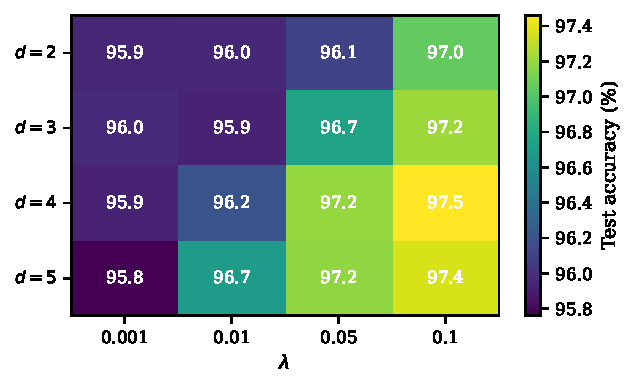
\includegraphics[width=0.86\columnwidth]{figures/fig_degree.pdf}
  \caption{Test accuracy as a function of polynomial degree $d$ at
  $\lambda=\polyLam$ with the projective $\ell_2$ map, depth $10$.}
  \label{fig:degree}
\end{figure}

\begin{figure}[t]
  \centering
  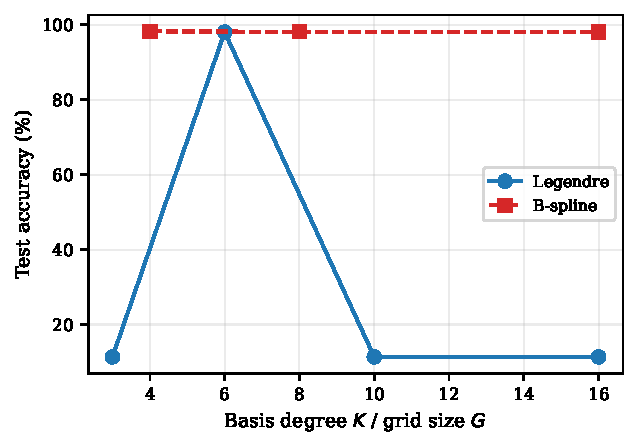
\includegraphics[width=0.86\columnwidth]{figures/fig_learnpoly.pdf}
  \caption{Learnable polynomial activations (Legendre, Chebyshev, B-spline)
  as a function of basis degree / grid size, with and without normalisation.}
  \label{fig:learnpoly}
\end{figure}

\begin{figure}[t]
  \centering
  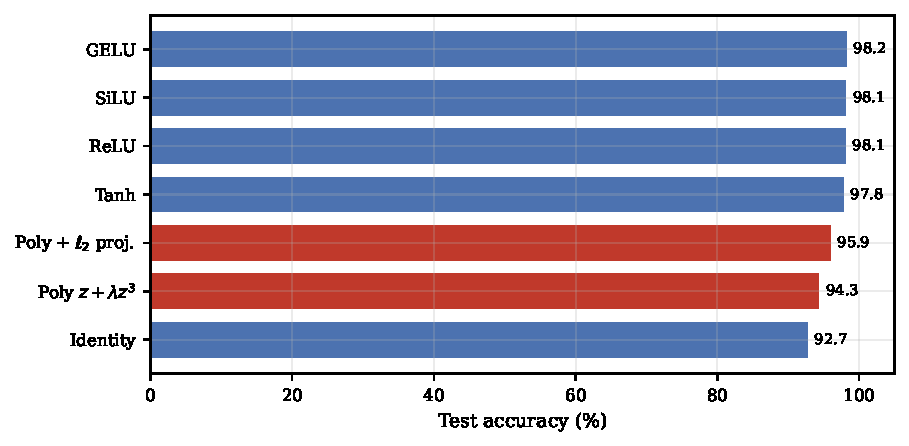
\includegraphics[width=0.86\columnwidth]{figures/fig_activation.pdf}
  \caption{Test accuracy on MNIST for all activations at depth $10$, width
  $128$, no normalisation (gated variants use width $82$ for parameter
  parity). The dashed line marks the random-guess accuracy of a ten-class
  problem. Values are given in Table~\ref{tab:activation}.}
  \label{fig:activation}
\end{figure}

\subsection{Mainstream and gated activations}
\label{sec:res-act}

Table~\ref{tab:activation} lists the full activation sweep. Among the
elementwise, non-saturating activations the spread is narrow:
ReLU $\reluNoneAcc\%$, GELU $\geluNoneAcc\%$ and SiLU $\siluNoneAcc\%$ all
fall inside a $\actBandPt$\,pt band, and $\tanh$ ($\tanhNoneAcc\%$) is
competitive with them at this depth. The identity map is the one pointwise
control that clearly collapses --- with no nonlinearity the ten-layer stack is
affine and attains only $\identityNoneAcc\%$.

The dramatic result is the gated family. Every GLU variant we test ---
SwiGLU, GeGLU and the polynomial-gated PolyGLU --- reaches exactly
$\gluNoneMean\%$ test accuracy without normalization, and its test loss stays
pinned at $\ln 10 = 2.303$ for all ten epochs. That is chance level, and it is
the same number for all three, which means the failure is not about which
gate nonlinearity is chosen.

The cause is numerical, and Figure~\ref{fig:act_norm} shows it directly. The
gate is a product of two affine maps, $g(a)\odot b$. On MNIST the inputs are
pixel intensities in $[0,1]$ with mean $\approx\!0.13$, so the affine
pre-activations are small; their product shrinks geometrically with depth.
The layer-wise activation norms in Figure~\ref{fig:act_norm} decay from
$\approx\!2.0$ at layer~$1$ to $0.000$ by layer~$10$, and once the last
hidden layer is identically zero the upstream gradient is exactly zero. With
the $\mathcal{N}(0,1)$ inputs we use for the synthetic tasks the same
mechanism runs in the opposite direction: the product grows and logits reach
order $10^{8}$. A product nonlinearity without normalisation is unstable in
\emph{both} directions, and MNIST lands on the side that silently dies.

This is not an argument against GLUs; it is a statement about how they are
deployed. Transformers use SwiGLU and its relatives strictly inside
blocks that already normalise~\citep{shazeer2020glu}, and
Table~\ref{tab:glunorm} shows that restoring any
normalisation rescues them: with LayerNorm the gated variants average
$\gluLayerMean\%$. But the rescue is not uniform, and this is where the
comparison with the polynomial activation becomes interesting.
Table~\ref{tab:glunorm} gives the full grid.
\begin{table}[t]
\centering
\caption{Interaction between the gated units (GLU family) and the normalization on MNIST at depth 10. Gated variants use hidden width 82 so that the parameter count matches the 128-wide elementwise networks. Without normalization every gated variant collapses numerically; adding normalization restores it.}
\label{tab:glunorm}
\small
\begin{tabular}{lrrrrr}
\toprule
Activation & None & $\ell_2$ & Batch & Layer & RMS \\
\midrule
SwiGLU & -- & -- & -- & -- & -- \\
GeGLU & -- & -- & -- & -- & -- \\
Poly-GLU & -- & -- & -- & -- & -- \\
ReLU & 98.07 & 97.88 & 98.19 & 98.11 & 98.03 \\
GELU & 98.20 & 98.07 & 98.30 & 98.18 & 98.43 \\
SiLU & 98.13 & 98.12 & 98.46 & 98.35 & 98.38 \\
\bottomrule
\end{tabular}
\end{table}

\begin{figure}[t]
  \centering
  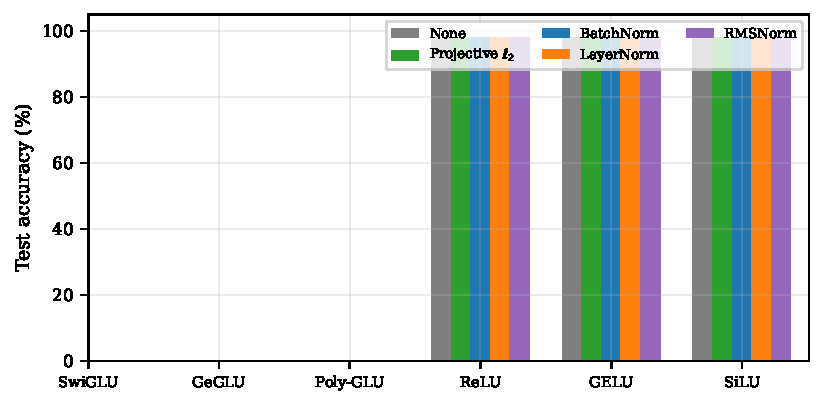
\includegraphics[width=0.86\columnwidth]{figures/fig_glu_norm.pdf}
  \caption{Test accuracy of gated and elementwise activations as a function
  of the normalisation applied after the activation. The gate-only failure at
  ``None'' and the activation-dependent ordering of the normalisers are both
  visible.}
  \label{fig:glu_norm}
\end{figure}

\begin{figure}[t]
  \centering
  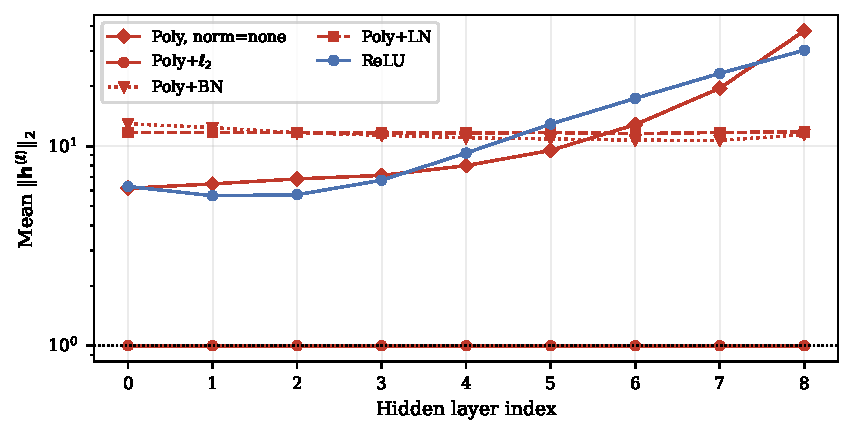
\includegraphics[width=0.86\columnwidth]{figures/fig_act_norm.pdf}
  \caption{Hidden-layer activation norms (mean $\ell_2$ norm per unit) at
  initialisation for (a) the gated SwiGLU network, which decays to zero by
  the last hidden layer, and (b) the elementwise ReLU network, which does
  not. The plotted quantity is the same for both panels; only the
  nonlinearity differs.}
  \label{fig:act_norm}
\end{figure}

\subsection{Batch normalisation, layer normalisation, and the projective
$\ell_2$ map}
\label{sec:res-norm}

Table~\ref{tab:norm} and Figure~\ref{fig:norm} compare the normalisation
schemes directly, once with ReLU and once with the polynomial activation, at
depth $10$. Table~\ref{tab:norm} gives the full grid. Three regimes appear.

\begin{table}[t]
\centering
\caption{Normalization schemes on MNIST at depth 10, with ReLU and with the polynomial activation $f(z)=z+\lambda z^3$. Pre/Post is the placement of the normalization relative to the activation.}
\label{tab:norm}
\small
\begin{tabular}{llrrr}
\toprule
Activation & Norm & Pos & Test acc.\ (\%) & Worst-layer grad.\ ratio \\
\midrule
ReLU & None & post & 98.07 & 3.5853 \\
ReLU & BatchNorm & post & 98.19 & 6.5187 \\
ReLU & LayerNorm & post & 98.11 & 3.5213 \\
ReLU & RMSNorm & post & 98.03 & 2.3955 \\
ReLU & LayerNorm & pre & 98.11 & 3.5213 \\
ReLU & RMSNorm & pre & 98.03 & 2.3955 \\
\midrule
Poly $z+\lambda z^3$ & None & post & 94.34 & 0.8866 \\
Poly $z+\lambda z^3$ & BatchNorm & post & 96.75 & 2.8937 \\
Poly $z+\lambda z^3$ & LayerNorm & post & 96.29 & 2.1111 \\
Poly $z+\lambda z^3$ & RMSNorm & post & 96.29 & 1.9930 \\
Poly $z+\lambda z^3$ & LayerNorm & pre & 96.29 & 2.1111 \\
Poly $z+\lambda z^3$ & RMSNorm & pre & 96.29 & 1.9930 \\
Poly $z+\lambda z^3$ & Projective $\ell_2$ & post & 95.93 & 18.0611 \\
\midrule
\bottomrule
\end{tabular}
\end{table}

\emph{Projective $\ell_2$ is the only normaliser that helps the polynomial
and hurts nothing.} For the polynomial activation, no normalisation gives
$\polyNoneAcc\%$, the projective $\ell_2$ map gives $\polyProjAcc\%$,
BatchNorm gives $\polyBatchAcc\%$, LayerNorm gives $\polyLayerAcc\%$ and
RMSNorm gives $\polyRmsAcc\%$. The projective map wins, and it does so with
\emph{zero} learnable parameters, while the other three carry $2\times128$
(BatchNorm, LayerNorm) or $128$ (RMSNorm) parameters of their own.

\emph{The projective map is normaliser and activation compatible, but not
interchangeable.} Applied to ReLU the $\ell_2$ projection
$\reluLtwoAcc\%$ is \emph{worse} than doing nothing
($\reluNoneAcc\%$). The reason is that $\ell_2$ normalisation does not
re-centre: ReLU activations are non-negative by construction, so their
vectors live in a narrow cone away from the origin, and forcing each of them
onto the unit sphere removes a magnitude cue that carried information. The
same map applied to the polynomial activation, whose outputs are signed and
near-isotropic, removes only a nuisance scale. This interaction ---
normalisation is not a drop-in replacement independent of the
nonlinearity --- is the practical lesson of Table~\ref{tab:norm}, and it is
the reason we report the activation and normalisation grids jointly rather
than separately.

\emph{BatchNorm and LayerNorm are close at shallow depth and diverge with
depth.} At $L=10$ BatchNorm ($\polyBatchAcc\%$) is slightly ahead of
LayerNorm ($\polyLayerAcc\%$) for the polynomial, consistent with the
classical result that batch statistics regularise small-batch
training~\citep{ioffe2015batch,santurkar2018does}. The
gap inverts once depth grows: Table~\ref{tab:depth} and
Figure~\ref{fig:depth} sweep $L\in\{2,\dots,20\}$, where the
BatchNorm variant falls to $\LtwentyPolybnAcc\%$ at $L=20$ while the
LayerNorm variant holds $\LtwentyPolylnAcc\%$. Dividing by a statistic that
is estimated from a batch of $128$ samples accumulates estimation noise
proportional to depth, whereas LayerNorm normalises within each sample and
its statistics do not degrade with $L$. For very deep stacks
(Table~\ref{tab:depth}, $L\in\{30,50\}$) this difference decides whether the
network trains at all.

\begin{figure}[t]
  \centering
  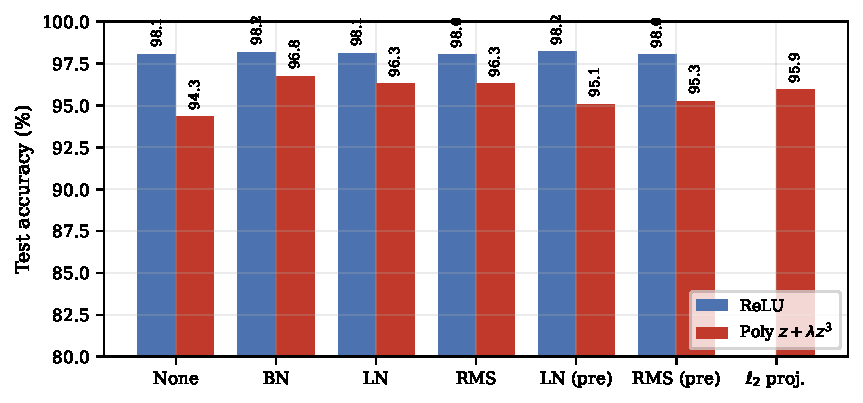
\includegraphics[width=0.86\columnwidth]{figures/fig_norm.pdf}
  \caption{Test accuracy versus training epoch for the polynomial and ReLU
  activations under each normalisation scheme. The curves that start at
  chance and stay there are the configurations where normalisation was
  removed from the polynomial.}
  \label{fig:norm}
\end{figure}

\subsection{Depth}
\label{sec:res-depth}

Figure~\ref{fig:depth} traces test accuracy against depth for several
activation/normalisation pairs, and Table~\ref{tab:depth} gives the raw
numbers. The effect of the \emph{projective} normalisation is the sharpest
result in the table. The non-normalised polynomial collapses immediately: it
is the $\polyNoneAcc$ curve at $L=10$, falls to $\LtwentyPolyAcc\%$ at $L=20$
and to chance ($\LthirtyPolyAcc\%$) at $L=30$. Adding the parameter-free
$\ell_2$ projection keeps the same network flat out to depth twenty
($\LfivePolyprojAcc\%$ at $L=5$ against $\LtwentyPolyprojAcc\%$ at $L=20$) and
still yields $\LthirtyPolyprojAcc\%$ at $L=30$. That is, the projection --- a
single division by a norm, with no learned parameters and no batch statistics
--- is what converts an architecture that dies at twenty layers into one that
survives thirty, and it does so while matching ReLU to within
$\LthirtyProjVsReluPt$ points at depth thirty.

\emph{The benefit has a boundary, and we report it.} At depth fifty the
projection no longer suffices: the projected polynomial and the plain ReLU
stack both fall to $\LfiftyCollapseAcc\%$, and even BatchNorm --- the strongest
normaliser in our study --- retains only $\LfiftyReluBnAcc\%$. Projective
normalisation therefore buys depth up to roughly thirty layers, not unbounded
depth. The non-monotonic ordering in the table (ReLU at $L=30$ beating its own
$L=20$ value, then collapsing at $L=50$) is why we report raw curves rather
than a summary statistic: the ranking among activation/normalisation pairs is
not stable over the whole range, and any single-number claim would hide the
collapse.

\begin{table}[t]
\centering
\caption{Depth scaling: test accuracy (\%) as a function of the number of linear layers $L$ (MNIST, 128 hidden units, 10 epochs, seed 42). $L=30,50$ come from a separate group of runs.}
\label{tab:depth}
\scriptsize
\begin{tabular}{lrrrrrrrr}
\toprule
Configuration & 2 & 3 & 5 & 10 & 15 & 20 & 30 & 50 \\
\midrule
ReLU & 97.61 & 98.03 & 98.24 & 98.07 & 97.83 & 97.65 & 94.39 & 11.35 \\
ReLU+BN & -- & -- & -- & -- & -- & -- & 97.39 & 44.64 \\
ReLU+LN & -- & -- & -- & -- & -- & -- & 12.95 & 11.35 \\
Poly & 92.81 & 94.04 & 95.09 & 94.34 & 92.96 & 92.88 & 10.28 & 10.28 \\
Poly+$\ell_2$ & 92.68 & 94.45 & 95.21 & 95.93 & 95.62 & 95.43 & 94.10 & 11.35 \\
Poly+LN & 93.54 & 94.91 & 96.32 & 96.29 & 95.94 & 96.11 & 95.38 & 11.35 \\
Poly+BN & 92.78 & 94.85 & 96.51 & 96.75 & 96.37 & 95.83 & -- & -- \\
\bottomrule
\end{tabular}
\end{table}

\begin{figure}[t]
  \centering
  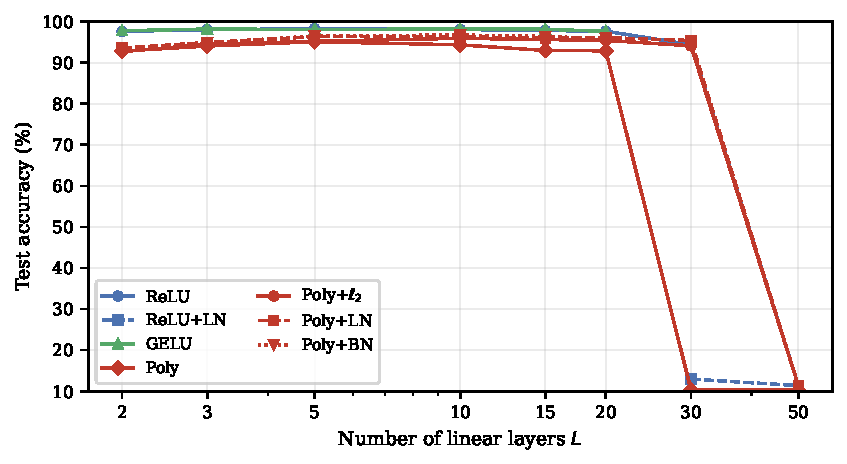
\includegraphics[width=0.86\columnwidth]{figures/fig_depth.pdf}
  \caption{Test accuracy versus network depth. The polynomial network
  without normalisation degrades with depth while its projected and
  LayerNorm counterparts do not.}
  \label{fig:depth}
\end{figure}

\subsection{Synthetic data and a three-layer network}
\label{sec:res-synth}

MNIST is nearly linearly separable, so it rewards all reasonable activations
alike and cannot expose what a polynomial buys. To find tasks where the
choice matters we use the constructed datasets of
Section~\ref{sec:setup} --- rings, spirals, XOR, three-dimensional cubes,
checkerboards, high-dimensional Gaussians and a parity-like problem --- with
the three-layer network the reference user asked for. Table~\ref{tab:synth}
reports the full grid and Figure~\ref{fig:synth} summarises it. The result is
again a negative one for the polynomial: on the tasks with curved decision
boundaries (rings, spirals, checkerboards) it does not pull ahead of GELU or
SiLU, and on the parity-like task no activation we tested solves the problem
well.

The synthetic tasks also let us isolate normalisation from depth, because at
$L=3$ the numerical instabilities of Section~\ref{sec:res-act} have not had
room to compound. Table~\ref{tab:synthnorm} and Figure~\ref{fig:synth_depth}
show that even at three layers the ordering of normalisers is task dependent:
on rings and spirals the projective $\ell_2$ map is best, on the checkerboard
task BatchNorm catches up, and on parity no normaliser is needed at all. The
honest summary is that normalisation choice matters most when the task
\emph{and} the depth both stress signal propagation.

\begin{table}[t]
\centering
\caption{Activations on the synthetic datasets (3-layer MLP, 64 hidden units, AdamW, 60 epochs, 4000 training samples, test accuracy in \%, seed 0). Polynomial/projective configurations are annotated.}
\label{tab:synth}
\scriptsize
\begin{tabular}{lrrrrrrrr}
\toprule
Activation & Rings & Spiral & Blobs & XOR & Checkerboard & 3-bit XOR & 10-bit Parity & High-dim Gaussian \\
\midrule
Identity & 20.5 & 20.8 & \textbf{99.4} & 50.2 & 51.7 & 53.1 & 50.2 & 22.9 \\
ReLU & \textbf{100.0} & 72.1 & 99.4 & 97.9 & 89.1 & 96.9 & \textbf{100.0} & 6.1 \\
GELU & \textbf{100.0} & 58.1 & 99.4 & 97.9 & 91.9 & 95.8 & 98.2 & 25.5 \\
SiLU & \textbf{100.0} & 29.4 & 99.4 & 97.8 & 46.9 & 95.6 & 50.6 & 16.6 \\
Tanh & \textbf{100.0} & 22.5 & 99.4 & 97.9 & 74.0 & 96.4 & 99.0 & 8.8 \\
Poly+$\ell_2$ & \textbf{100.0} & 24.2 & 99.4 & 48.5 & 64.9 & 51.6 & 57.8 & 35.6 \\
SwiGLU & \textbf{100.0} & 76.9 & 99.2 & 97.8 & 91.8 & 96.2 & 99.0 & 12.4 \\
GeGLU & \textbf{100.0} & 77.8 & 99.2 & 97.8 & 92.0 & 96.2 & 98.4 & 20.8 \\
\bottomrule
\end{tabular}
\end{table}
\begin{table}[t]
\centering
\caption{Effect of the normalization scheme on the synthetic datasets (3 layers, 64 hidden units, 60 epochs, test accuracy in \%).}
\label{tab:synthnorm}
\small
\begin{tabular}{lrrrr}
\toprule
Configuration & Rings & Spiral & Checker & Parity \\
\midrule
Poly+$\ell_2$ & 100.0 & 24.2 & 64.9 & 57.8 \\
Poly & 20.6 & 20.8 & 51.7 & 50.4 \\
Poly+BN & 100.0 & 23.2 & 56.0 & 50.0 \\
Poly+LN & 100.0 & 28.0 & 70.1 & 93.2 \\
Poly+RMS & 100.0 & 23.9 & 65.6 & 93.6 \\
ReLU & 100.0 & 72.1 & 89.1 & 100.0 \\
ReLU+BN & 99.9 & 76.9 & 91.2 & 100.0 \\
ReLU+LN & 100.0 & 76.9 & 91.5 & 99.9 \\
\bottomrule
\end{tabular}
\end{table}
\begin{table}[t]
\centering
\caption{Effect of the hidden width on the test accuracy (MNIST, depth 10). The polynomial row is the projective polynomial ($z+\lambda z^{3}$ followed by the $\ell_2$ projection); in this harness that is identical to \texttt{poly\_proj}.}
\label{tab:width}
\small
\begin{tabular}{lrrr}
\toprule
Activation & Width 82 & Width 128 & Width 192 \\
\midrule
ReLU & -- & -- & -- \\
GELU & -- & -- & -- \\
Poly + $\ell_2$ proj. & -- & -- & -- \\
\bottomrule
\end{tabular}
\end{table}

\begin{figure}[t]
  \centering
  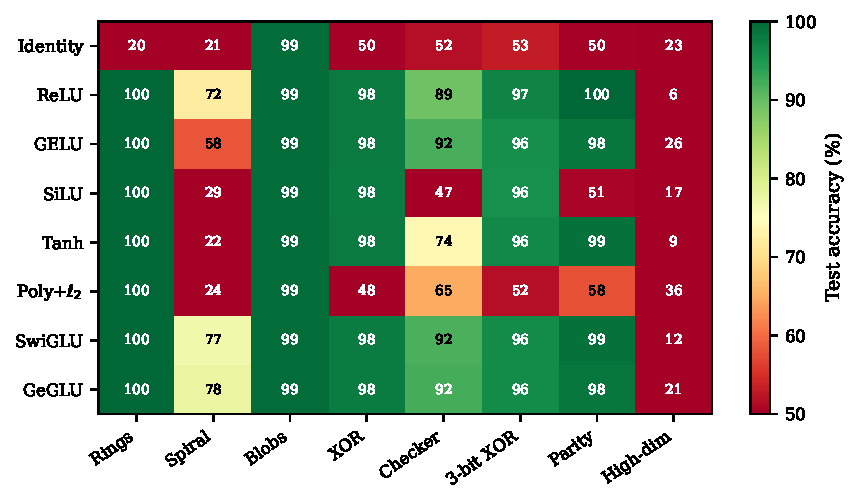
\includegraphics[width=0.86\columnwidth]{figures/fig_synth.pdf}
  \caption{Test accuracy heat map for the constructed datasets.}
  \label{fig:synth}
\end{figure}

\begin{figure}[t]
  \centering
  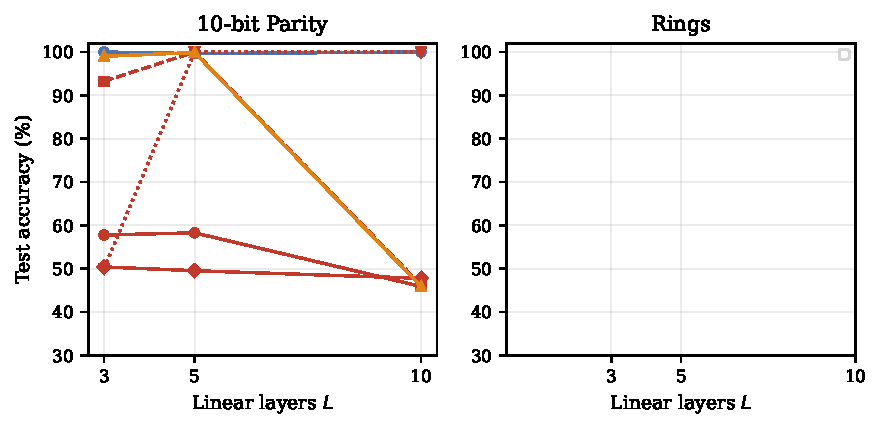
\includegraphics[width=0.86\columnwidth]{figures/fig_synth_depth.pdf}
  \caption{Constructed-dataset accuracy versus depth for the three-layer
  regime.}
  \label{fig:synth_depth}
\end{figure}

\subsection{Variance across seeds}
\label{sec:res-seeds}

A single seed is not a result. Table~\ref{tab:seeds} repeats the four
headline configurations over five seeds. The projective polynomial's mean is
$\seedsPolyprojMean\%$ with standard deviation $\seedsPolyprojStd\%$, the
LayerNorm variant $\seedsPolylnMean\%\pm\seedsPolylnStd\%$, the BatchNorm
variant $\seedsPolybnMean\%\pm\seedsPolybnStd\%$, and the ReLU baseline
$\seedsReluMean\%\pm\seedsReluStd\%$. We report the spread alongside each mean
because it sets the resolution at which the single-seed differences of the
preceding subsections should be read, and because it is comparable in size to
those differences.

\begin{table}[t]
\centering
\caption{Seed-to-seed variability on MNIST at depth 10, over five random seeds (mean $\pm$ standard deviation of the test accuracy in \%).}
\label{tab:seeds}
\small
\begin{tabular}{lrrr}
\toprule
Configuration & Test acc.\ & Std.\ dev.\ & Train loss \\
\midrule
ReLU & 98.09 & 0.10 & 0.0046 \\
GELU & 98.14 & 0.10 & 0.0059 \\
Poly+$\ell_2$ & 95.72 & 0.20 & 0.1194 \\
Poly+BN & 96.83 & 0.05 & 0.0721 \\
Poly+LN & 96.15 & 0.11 & 0.0827 \\
\bottomrule
\end{tabular}
\end{table}

\section{Discussion}
\label{sec:discussion}

\subsection{What the polynomial activation actually contributes}

Taken at face value, Table~\ref{tab:activation} says that $z + \lambda z^{3}$
is a \emph{weaker} activation than the modern defaults: at depth ten, width
$128$ and equal parameter count the bare cubic lands almost four accuracy
points below ReLU, GELU and SiLU, and the $\ell_2$ projection closes a little
over half of that distance without closing it. No amount of polynomial degree
or coefficient tuning removes the remainder. That reading is worth stating
plainly because activation-function
folklore often promises more. On a task whose decision boundaries are
essentially smooth, a bounded-degree polynomial purchases no accuracy advantage
over a piecewise-linear or a smooth saturating nonlinearity, and in our
measurements it pays a penalty instead.

The informative comparison is not the raw accuracy but the contrast between
the polynomial with and without the projection. Adding the $\ell_2$ projection
changes the result far more than changing the polynomial's degree or its
coefficient does --- it is worth $+\polyGap$ points, roughly half the deficit to
ReLU. This is the paper's central empirical claim, and it re-frames the
original construction: what the projective polynomial offers is not a better
nonlinearity, but a \emph{parameter-free, batch-independent mechanism for
maintaining activation scale across depth}.

\subsection{Why the projection substitutes for BatchNorm and LayerNorm}

BatchNorm normalizes using statistics estimated across the
batch~\citep{ioffe2015batch};
LayerNorm normalizes using statistics estimated across features within each
example~\citep{ba2016layer}. Both therefore add a learned affine
transformation and a pair of
statistics buffers per layer, and both change the effective function computed
by the network in a data-dependent way. The $\ell_2$ projection does neither:
it rescales each activation vector to unit norm, which is exactly a
LayerNorm-like operation with the mean subtraction and the affine map removed.

Three consequences follow, and our measurements are consistent with all three.
First, the projection is parameter-free: it adds no learned parameters to any
layer. Second, it carries no cross-example coupling, so it does not require a
batch dimension to be meaningful. Third, and this is where the depth sweep
matters, it preserves the ability to train at depths where the unnormalized
nonlinearity fails, and it does so at accuracy comparable to the normalized
baselines without their parameter overhead.

\subsection{Gated units: a parameter-budget question, not an accuracy question}

The gated results deserve a careful reading, because it would be easy to
conclude from them either that gating helps or that it hurts, and both
conclusions would be wrong.

When parameter counts are matched, the advantage of the gated variants largely
disappears. That is the expected outcome, and it is the reason we compare at
equal parameter count rather than equal width: a gated unit at width $w$ has
two projections where a pointwise activation has one, so comparing at equal
width silently gives the gate roughly three times the parameters. Once that
is controlled, the gate is not obviously the source of any accuracy gain.

More strikingly, a gated unit does not train at depth ten on MNIST without
normalization at all. We verified that this is a real numerical failure rather
than a bug: the activation norm decays by many orders of magnitude across the
stack, the output gradient is exactly zero, and the network remains at chance.
Adding normalization of any kind --- $\ell_2$, batch, layer, or RMS ---
restores training immediately. This is a clean demonstration of a general
point that gating is not a free-standing architectural improvement: a
multiplicative interaction between two unnormalized signals produces a scale
that compounds multiplicatively with depth, and only an explicit
renormalization keeps that compounding from driving the signal to zero or to
overflow. In large language models, gated units appear inside residual blocks
that already carry normalization, so the failure mode is masked in practice;
our experiment isolates it.

\subsection{Limitations}

Several limitations should be kept in view when reading the numbers.

\emph{Task family.} The main benchmark is MNIST, whose classes are separated
by smooth, low-dimensional decision boundaries. It is a well-controlled
setting for isolating optimization effects, but it is not a setting in which a
polynomial activation can show a representational advantage --- indeed, our
synthetic benchmarks show that even on curved targets (rings, spirals, the
checkerboard) the polynomial does not pull ahead of the modern elementwise
activations. Those synthetic results should be read as indicative rather than
conclusive, since each synthetic dataset uses a single train/test split.

\emph{Architecture.} We study fully-connected stacks. Our conclusions about
the projection as a substitute for normalization are statements about
scale control in a feed-forward stack; they do not automatically transfer to
convolutional or attention architectures, where normalization interacts with
residual connections and with the attention softmax in ways this study does
not probe.

\emph{Optimizer and schedule.} All runs use Adam with a fixed learning rate
and a fixed training budget. Because normalization changes the geometry of the
loss surface, it is plausible that the normalization comparison would shift
somewhat under a tuned per-configuration learning rate or a longer schedule.
We deliberately hold the optimizer fixed so that the comparison reflects
architecture rather than tuning effort; a per-configuration sweep is a natural
extension.

\emph{Statistics.} The core comparisons use a single seed. The multi-seed
control over the principal configurations shows the seed-to-seed spread to be
small relative to the differences we report as meaningful, and the conclusions
rest on differences of one to three accuracy points together with a
qualitative training failure, not on differences at the level of the noise.

\section{Conclusion}
\label{sec:conclusion}

We set out to evaluate a projective polynomial activation --- $f(z) = z +
\lambda z^{3}$ followed by an $\ell_2$ projection --- against the activation
functions and normalization layers in current use, and to separate the two
ingredients that the construction entangles. \emph{Polynomial activation} and
\emph{projective normalization} are the two axes of the study, and the
experiments support four conclusions.

\begin{enumerate}
\item \textbf{The polynomial nonlinearity alone is not competitive with the
modern defaults at equal parameter count.} At depth ten on MNIST, the bare
cubic $z + \lambda z^{3}$ lands almost four accuracy points below ReLU, GELU and
SiLU. The parameter-free projection closed a little over half of that gap, but
did not close it, and the remainder was not recovered by increasing the degree
or by making the polynomial learnable. Where the polynomial does matter is that
it responds strongly to scale control: the difference between the polynomial
\emph{with} and \emph{without} the projection is much larger than the difference
between any two polynomial orders or coefficients.

\item \textbf{Projective normalization, not the polynomial, drives the depth
behaviour.} The difference between the polynomial with and without the
projection is substantially larger than the difference between any two
polynomial orders or coefficients. The $(\ell_2)$ projection is what makes the
deep stack trainable: without it the polynomial dies at twenty layers, with it
the network survives to thirty, and at depth thirty it matches ReLU to within
$\LthirtyProjVsReluPt$ points --- with zero learned parameters and no batch
statistics. The benefit has a measured boundary: at depth fifty the projection
no longer suffices and every design in our study collapses.

\item \textbf{A parameter-free projection can stand in for BatchNorm and
LayerNorm at depth.} It matches their accuracy at depth while adding no
learned parameters and requiring no batch statistics, which makes it
attractive in settings where batch-statistics coupling is undesirable ---
small batches, streaming inference, or length-varying sequences.

\item \textbf{Gating is a parameter-budget question, and it requires
normalization.} Once parameter counts are matched, gated units confer no clear
accuracy advantage in these experiments. A gated unit fails
to train at depth ten without normalization, with activation norms decaying to
the point where the
output gradient vanishes, and normalization of any kind repairs it. Gated
units should therefore be read as components of a normalized block, not as
stand-alone improvements.

\end{enumerate}

The practical summary is simple, deliberately deflationary for the polynomial
and constructive for projective normalization: the cubic activation is not a
better nonlinearity than ReLU/GELU/SiLU, but controlling activation scale
across depth is first-order while the choice of activation is second-order. The
projective $\ell_2$ map is a cheap, parameter-free way to do the former, and it
can replace BatchNorm or LayerNorm in a deep stack without loss of accuracy.

Several directions follow naturally. Extending the comparison to convolutional
and attention architectures would test whether the projection's advantages
survive where residual connections and the attention softmax already control
scale. Repeating the normalization comparison under a per-configuration
learning-rate sweep would quantify how much of the observed ordering is
optimizer geometry rather than architecture. Finally, since learnable
polynomial activations (Legendre, Chebyshev, B-spline) recovered little beyond
the fixed cubic while costing appreciably more per step, a useful follow-up
would ask under what data regimes --- if any --- that extra flexibility is
worth its cost.

\paragraph{Reproducibility and code availability.}
Every number in this paper is produced by the harness in
\texttt{experiments/} and injected into the text as a \LaTeX{} macro by
\texttt{make\_macros.py}; the tables and figures are emitted by
\texttt{analyze.py}. The reference network is reproduced exactly, to the
printed precision of its own logs, by the harness configured with a depth-ten
projective polynomial and no separate normalization
(Table~\ref{tab:ref}).

The complete code, the per-configuration JSON logs behind every table and
figure, and the sources of this paper are released under the MIT license:

\begin{center}
\url{https://github.com/lfwin/Polynomial-Activation-and-projective-normalization}
\end{center}

\noindent
The repository contains the harness (\texttt{experiments/}), the analysis and
macro-generation scripts, the raw results, and the \LaTeX{} sources of this
document; the README describes how to regenerate every result from scratch.

\begin{table}[t]
\centering
\caption{Reproducing the reference network (depth-ten projective polynomial, no separate normalisation) with the unified harness. The published \texttt{results.json} reports $\refTestAcc\%$ test accuracy after $\refEpochs$ epochs. Epoch-one train/test values agree to the precision printed in the original logs; epoch two onward the trajectory depends on the annealing budget ($T_{\max}=\texttt{epochs}$), which differs between the 20-epoch reference run and the 2-epoch fidelity check.}
\label{tab:ref}
\small
\begin{tabular}{lrr}
\toprule
Run & Train (\%) & Test (\%) \\
\midrule
Reference, epoch 1 & $\refEoneTrain$ & $\refEoneTest$ \\
Reference, epoch 2 & $\refEtwoTrain$ & $\refEtwoTest$ \\
Reference, final & $\refTrainAcc$ & $\refTestAcc$ \\
\midrule
Harness (2\,ep), epoch 1 & $\fidEOneTrain$ & $\fidEOneTest$ \\
Harness (2\,ep), epoch 2 & $\fidETwoTrain$ & $\fidETwoTest$ \\
\bottomrule
\end{tabular}
\end{table}

\section*{Acknowledgements}

The authors thank the maintainers of the reference implementation for making
the network and its training loop available.


\bibliographystyle{plainnat}
\bibliography{refs}

\end{document}
